%\graphicspath{Figures/detector}

\chapter{The \LHC and \CMS experiment}
\label{chap:detector}

\chapterquote{Insanity: doing the same thing over and over again and expecting different results.}
{Albert Einstein, 1879 –- 1955}

Probing the physics of the \ac{SM} and beyond at the~\TeV scale is only possible with the technologically unparalleled apparatus situated at the \ac{CERN}.
This chapter will introduce the hugely complex machinery of the \LHC, 
which provides proton-proton collisions at energies in excess of $\sqrt{7}$~\TeV, 
and outline the main features of the \ac{CMS} experiment, of which the author is a member, 
with particular focus on those features relevant to the material presented in this thesis.
%exploited in the search for new physics using monojet events.
%
Section~\ref{sec:LHC} presents the main features of the \ac{LHC}, and Section~\ref{sec:CMS} provides an overview of the \ac{CMS}  detector. 

%%%%%%%%%%%%%%%%%%%%	LHC	%%%%%%%%%%%%%%%%%%%%%%%%%%%%

\section{The \LHC}
\label{sec:LHC}
The \ac{LHC} is the world's largest and most energetic synchrotron particle collider. 
Housed in the tunnel built for the \ac{LEP} collider that operated during the 1990's at \ac{CERN}, 
the \ac{LHC} is a double ring circular collider 27~\km in circumference, 
and sits on the bedrock beneath the Franco-Swiss border, close to Geneva, Switzerland. 
It is designed for both proton-proton (pp) and heavy ion (PbPb) collisions at a centre of mass energy $\sqrt{s} = 14~\TeV$ and luminosity of \designLumi.


Currently the world's only operating collider able to study physics at the~\TeV scale, the \ac{LHC} consists of thousands of superconducting magnets which act to accelerate, bend and focus two beams of protons (or heavy ions) that circulate in opposite directions around the accelerator. 
%injector chain
A chain of accelerators, culminating with the \ac{SPS}, inject bunches of approximately one hundred billion protons 25 or 50~\ns apart at $\sqrt{s} = 450~\GeV$ into the two beams of \ac{LHC}.
Oscillating electric fields provided by 1232 superconducting dipole magnets act to accelerate the beams up to the operating centre of mass energy, which for the data used in this thesis was $\sqrt{s} = 8$~\TeV, with bunch crossings every 50~\ns.
Once protons are accelerated to the operational $\sqrt{s}$, the \ac{LHC} acts as a storage ring, and collisions can occur.
%
Either side of four points around the \ac{LHC} ring, very high precision magnetic fields, provided by quadrupole and higher order multipole magnets, position and focus the beams such that each bunch has a diameter of 16~$\mu$m. 
The chance of a pp collision with large momentum transfer at the four interaction points around the LHC ring is thereby increased, and the number of such collisions per bunch crossing, termed ``pile-up'' (PU) for the data used in this thesis was $\sim20$.

%picture
\begin{figure}[htbp]
  \begin{center}
  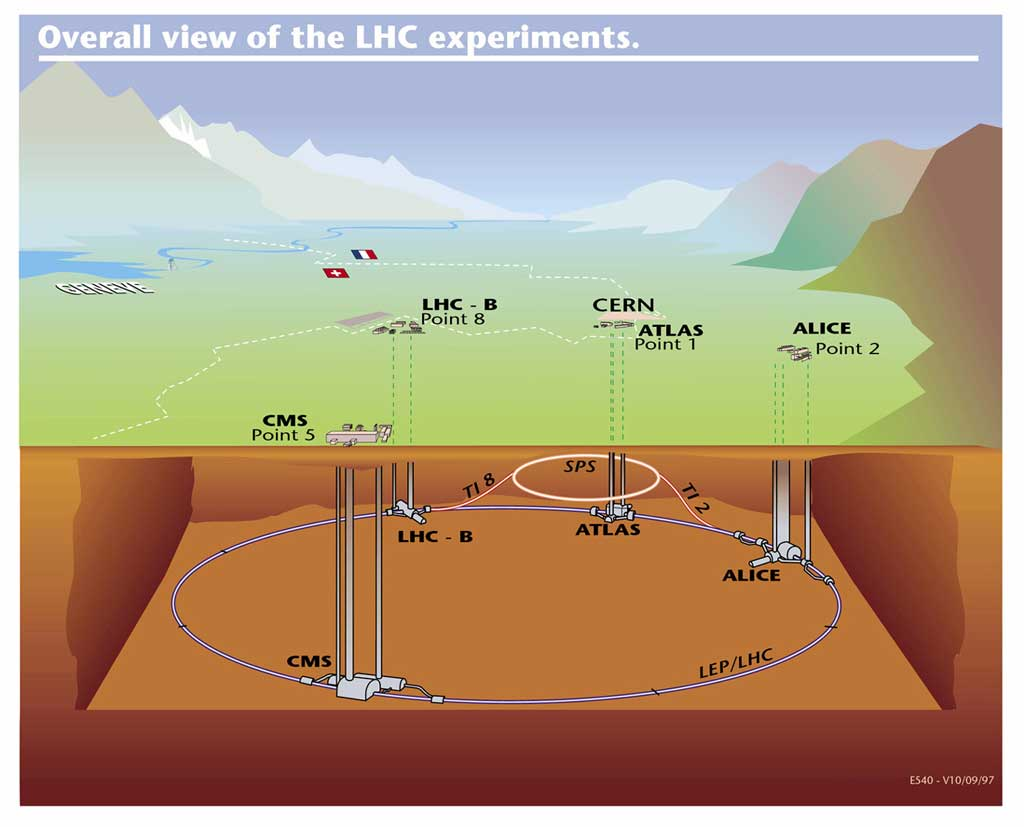
\includegraphics[width=0.8\textwidth]{Figures/detector/LHCdesign}
  \caption{The ~\LHC accelerator ring, showing the locations of the four main experiments at the four collision points.
}
  \label{fig:LHC}
  \end{center}
\end{figure}

Interaction points are at the centre of four large particle detectors, shown in Figure~\ref{fig:LHC}:
A Large Ion Collider Experiment (\ALICE)~\cite{Aamodt:2008zz}, 
A Large Toroidal LHC ApparatuS (\ATLAS)~\cite{Aad:2008zzm}, 
Compact Muon Solenoid (\CMS)~\cite{Chatrchyan:2008aa} and 
Large Hadron Collider Beauty (\LHCb)~\cite{Alves:2008zz}.
They act to identify particles produced as a result of a pp or PbPb bunch crossing through a combination of tracking and calorimetry, in order to reconstruct and measure physical processes, to test currently accepted theories and search for new physics.

%running in Run 1

\section{The CMS Detector}
\label{sec:CMS}

The \ac{CMS} detector is a general purpose particle detector, designed to carry out many different measurements for various physics goals.
Close to 4$\pi$ reconstruction with 
efficient particle identification and reconstruction allows measurements of photons, muons, electrons, taus, hadronic showers and missing transverse momentum.
%It is therefore very well suited to the search for new physics, and direct production of \ac{SUSY}, in many different forms.
%Here, we focus on the search for new physics, particularly using the monojet final state.
%
A diagram of \ac{CMS} is shown in Figure~\ref{fig:CMS}. It is 21.6~\m long, 14.6~\m in diameter and weighs 12500~T. 
It consists of different sub-detectors, each of which measures a different particle or property, 
and is built around a central 12.5~m long 4~\T superconducting solenoid magnet and its iron return yoke.
%
\ac{CMS} consists of a barrel region, containing the solenoid, and endcaps to extend the forward and backward coverage.

%
The different sub-detectors are arranged in an onion structure.
%
Closest to the beam line is the silicon tracking system.
A very highly resolution pixel detector lies closest to the interaction region, followed by a granular strip detector.
Charged particle momenta measurements are made using the curvature of tracks in the uniform magnetic field provided by the solenoid, as well as measurements of displaced vertices and impact parameters which are essential for identifying heavy flavor decays. 
%
Energy measurements are provided by the calorimeters, which lie outside of the tracker; the \ac{ECAL} and \ac{HCAL}. 
The highly granular \ac{ECAL} consists of 70,000 transparent lead tungstate crystals, which allow accurate electron and photon position and energy measurements. 
Scintillation light produced in the crystals is collected by photodetectors and used to infer the incident particle energy.
%
The sampling \ac{HCAL} consists of slabs of brass interleaved with plastic. 
Hadron showers are produced in the absorber (brass) and scintillation light is produced in the active material (plastic) as the shower passes through.
%
The solenoid lies outside of the \ac{HCAL} and provides a 3.8~\T axial magnetic field.
%
Embedded in the iron return yoke of the magnet sit the muon systems. 
Three different types of muon detectors are used to identify muons and make momentum and charge measurements over a large kinematic range.
%

%
Crucial to the successful operation of \ac{CMS} is the trigger. 
The pp interaction cross section is 100~\mb, while for example, the W boson production cross section is some 6 orders of magnitude less than this, and the rare physics processes that \ac{CMS} was built to search for, such as Higgs boson and \ac{SUSY} production, many times smaller still.
The \ac{LHC} delivers an unprecedented high instantaneous luminosity so that such rare physics processes occur, but this also implies that the vast majority of the collisions result in `uninteresting' physics: namely \ac{QCD} processes.
It would be impossible to record such high volumes of data that comes out of \ac{CMS}, some PB s$^{-1}$, and not useful to do so.
Therefore, a very efficient method of recording those events that appear `interesting'  
is necessary, to reduce the 40~\MHz event rate to a more manageable 100~\Hz.
The two-tier trigger system fulfills this role, via a hardware based online \ac{L1} an software based offline \ac{HLT}.

%
More information on the CMS detector can be found in Ref.~\cite{Chatrchyan:2008aa}.

%%%%%%%
% Inside the solenoid and closest to the beam line is the tracking system.
% In the uniform magnetic field provided by the solenoid, charged particles leave curved tracks 
% in the component silicon pixels and strips, under the influence of the Lorentz force.
% Momenta measurements are made by measuring the curvature of these tracks.
% %
% The next subsystems out are the calorimeters: the \ac{ECAL} and \ac{HCAL}. 
% Consisting of absorber materials which cause electromagnetic and hadron showers, they totally absorb a particle, prompting scintillation light proportional to its energy in the active material. 
% An energy measurement is made by measuring the scintillation light and inferring the energy of the incident particle.
% %
% Finally, embedded in the return yoke of the magnet sit the muon systems. 
% Muons are relatively long lived, heavier and therefore more penetrating than other particles,
% so require detectors further away from the interaction point. 
% Three different types of muon detectors, interleaved with the steel return yoke of the solenoid, are used to identify muons and make momentum and charge measurements over a large kinematic range.
% %
% More information on the CMS detector can be found in Ref.~\cite{Chatrchyan:2008aa}.

%picture
\begin{figure}[htbp]
  \begin{center}
  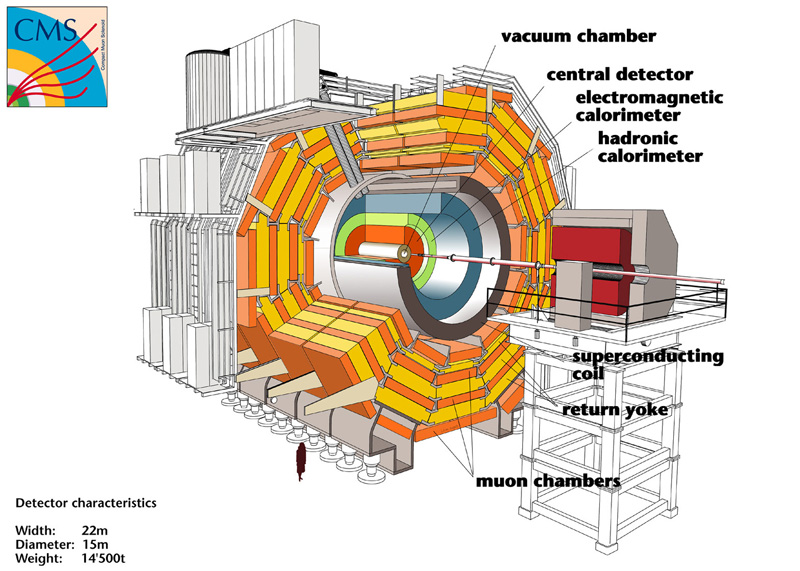
\includegraphics[width=0.8\textwidth]{Figures/detector/CMSlabelled}
  \caption{The \ac{CMS} detector, with the main subsystems labelled.
}
  \label{fig:CMS}
  \end{center}
\end{figure}

%coordinate system
\ac{CMS} uses a right-handed coordinate system; the $x$-axis points south towards the centre of the \ac{LHC} ring, the $y$-axis points vertically upwards and the $z$-axis is in the direction of the beam, where positive $z$ is to the west.
More useful is the cylindrical coordinate system, defined in terms of $r$, $\phi$ and $\theta$.
The azimuthal angle $\phi$ is measured from the $x$-axis in the $xy$ plane, where the radial component is denoted $r$. The polar angle $\theta$ is defined in the $rz$ plane, and the pseudorapity 
\begin{equation}
\eta = - \ln \tan (\theta /2).
\end{equation}
Convention is that the position of a particle is described in terms of $\eta$ and $\phi$, where $\eta = 0$ is along the $y$-axis and $\eta = \infty $ is along the beam direction; and $-\pi < \phi < \pi$. The distance between particles is commonly described in terms of the variable $\Delta R = \sqrt{\Delta\phi^2+\Delta\eta^2}$.

The \ac{LHC} is a hadron collider, and as such, collides non-fundamental particles. 
Inelastic collisions with large momentum transfer can occur between component quarks and gluons, however in a single bunch crossing there will also be many low energy, elastic, soft scatters, 
as well as the remnant part of any protons that have had a hard collision. 
As a result, the forward and backward directions are highly radiative environments and therefore difficult to instrument due to high occupancy and radiation damage. 
\ac{CMS} has endcaps to extend the detector coverage at high $\eta$, however it is not possible to reconstruct momentum of a single interaction in the direction of the beam.   
Additionally, interesting physics is a result of a hard collision, where energy is available for the creation of new particles. It can be characterized by the amount of energy in the transverse ($xy$) plane.
For these reasons, particle energy and momenta are described only in the transverse plane, where conservation laws can be applied.
By conserving energy and momentum in the transverse plane, any imbalance can be assigned to a particle leaving the detector without any trace; for example from a neutrino, or, from new physics processes such as \ac{DM} production.
4\pi particle reconstruction and measurements of missing transverse energy, the `tell-tale' sign of new physics, makes \ac{CMS} perfectly suited to searching for physics beyond the \ac{SM}.

%%%%%%%%%%%%%%%%%%%%%%%%%%%%%%%%%%%%%%%%%%%%%%%%%%%%%%%%%%%%%%%%%%%%%%%%

\subsection{The Tracking System}
The tracker is designed for precise and efficient measurement of charged particle trajectories (and therefore position and momentum) as they emerge from the interaction point.
Additionally, reconstruction of any secondary vertices is crucial for identifying heavy flavor decays such as jets that originate from b-quarks.

The \ac{LHC} provides bunch crossings every 25 or 50~\ns, resulting in $\sim$ 20 pp interactions, giving rise to of order 1000 particles. 
All of these traverse the tracker. 
The granularity of the tracker must be such that one can determine which of the $\sim$ 20 pp vertices each of the particles come from, 
and the electronics fast enough that the information is sent on in time for the next bunch crossing to arrive.
With such high particle fluxes, the tracker is also subject to a huge amount of radiation damage.
These conditions must be dealt with using the least amount of material possible in order to limit multiple scattering, photon conversion, bremsstrahlung and nuclear interactions.
To meet with such criteria, and to have an estimated lifetime of 10 years, the tracker is constructed entirely from silicon.

The tracker consists therefore of an all silicon pixel and strip detector.
Measuring 5.8~\m in length and 2.5~\m in diameter, with a total active area of 200~\msq, it surrounds the interaction region.
%pixel
The pixel detector has three layers in the barrel, at radii of 4.4~\cm, 7.3~\cm and 10.2~\cm. In the endcaps, there are two disks at distances $z=\pm 34.5, \pm 46.5~\cm$.
%strip
The strip detector has a length of 5.8~\m and a diameter of 2.4~\m, and is composed of four subsystems: the \ac{TIB}, \ac{TOB}, \ac{TID} and \ac{TEC}. The \ac{CMS} tracker geometry is shown in Figure~\ref{fig:CMStracker}.

%picture
\begin{figure}[htbp]
  \begin{center}
  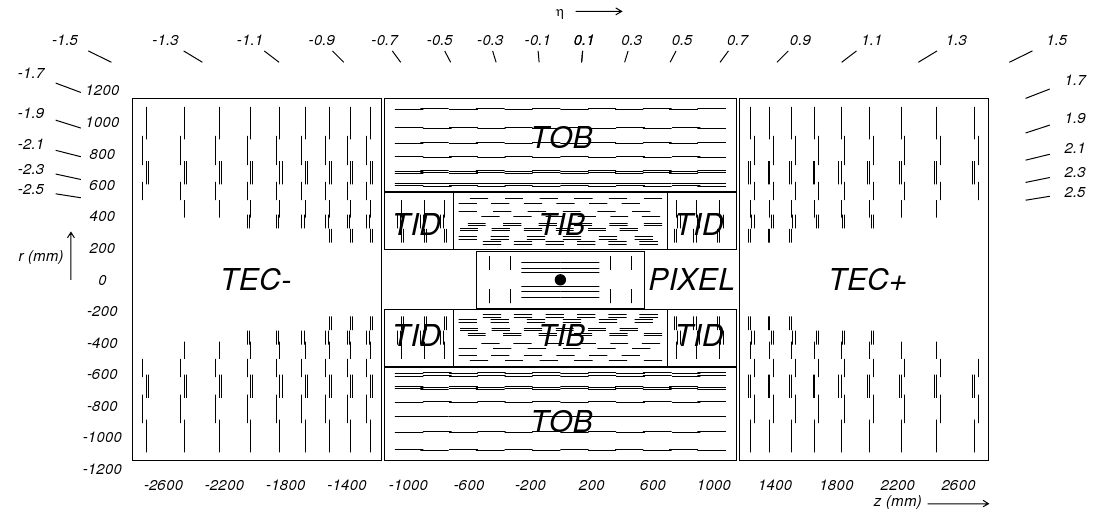
\includegraphics[width=0.9\textwidth]{Figures/detector/fig_cmstracker}
  \caption{The \ac{CMS} tracker, shown in the $rz$ plane. The pixel detector is shown at the centre of the tracker, closest to the interaction region (shown by the black dot), and the strip detector surrounds it. The different subsystems of the strip detector are shown, taken from Ref.~~\cite{Chatrchyan:2008aa}.
}
  \label{fig:CMStracker}
  \end{center}
\end{figure}

%%%%%%%%%%%%%%%%%%%%%%%%%%%%%%%%%%%%%%%%%%%%%%%%%%%%%%%%%%%%%%%%%%%%%

\subsection{The Electromagnetic Calorimeter}
High resolution photon and electron position and energy measurements are provided by the lead tungstate (PbWO$_{4}$) crystal \ac{ECAL}, which covers pseudorapidty up to $|\eta|<3$.
It is made up of the \ac{EB}, covering the range $0<|\eta|<1.479$,
and the \ac{EE}, covering the range $1.479<|\eta|<3$.

Both fast response times (80\% of scintillation light is emitted in 25~\ns) and radiation hardness are required from the \ac{ECAL}, motivating the choice of material.
In addition, it is very dense (8.28~g$\cm^{-1}$), has a short radiation length ($X_{0} = 0.89~\cm$), and small Moli\`{e}re radius (2.2~\cm), making it well suited to a compact, fine granularity calorimeter.
61,200 crystals in the barrel and 7,324 crystals in the endcaps are tapered in shape and arranged in a quasi-projective geometry, angled at 3\deg to ensure that particle trajectories avoid cracks between them.
Barrel crystals have a front face of $22 \times 22$~mm$^{2}$ and a length of 23~\cm, corresponding to 25.8~$X_{0}$. 
Endcap crystals have a front face of $28.6 \times 28.6$~mm$^{2}$ and length corresponding to 24.7~$X_{0}$.
Electromagnetic showers are therefore expected to be contained within one crystal length, so only a single layer of crystals is needed. 
A preshower detector is place in front of the endcaps, with a thickness of $3X_{0}$, in the range $1.653<|\eta|<2.6$, in order to distinguish between single photons and photon pairs resulting from neutral pion decay. 
The \ac{ECAL} geometry is shown in Figure~\ref{fig:CMSecal}.

%picture
\begin{figure}[htbp]
  \begin{center}
  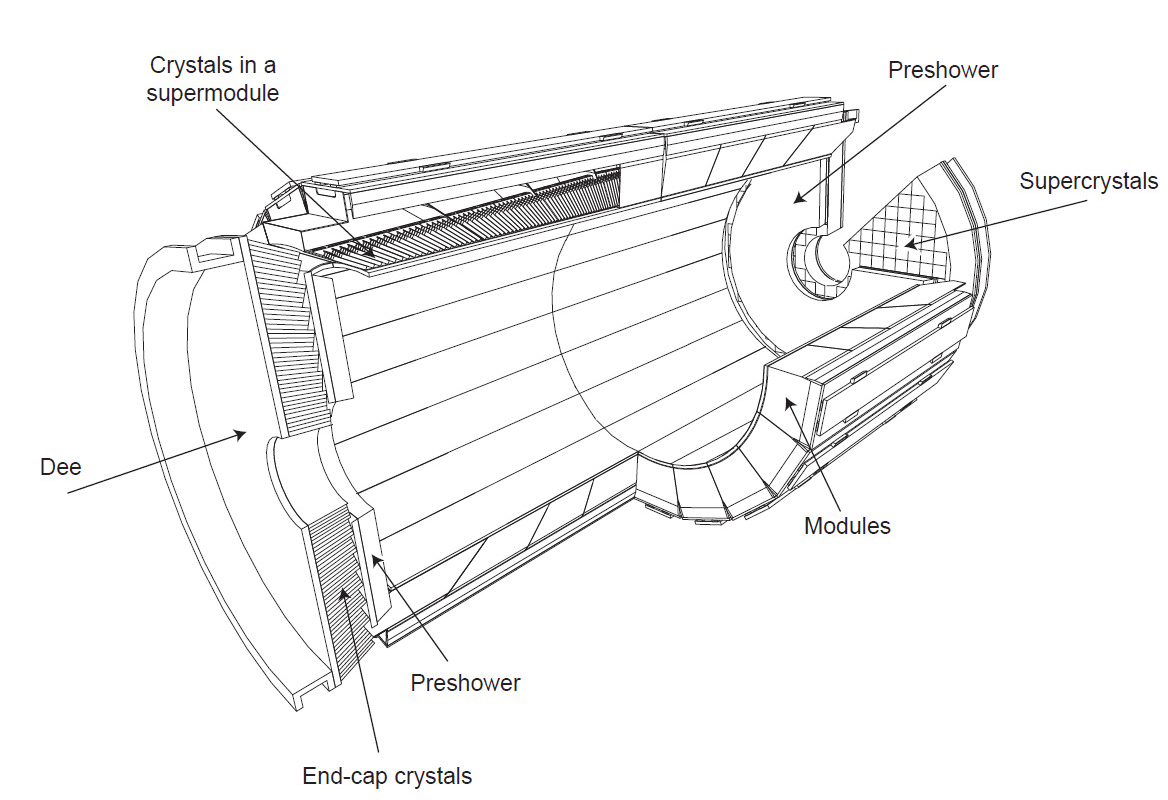
\includegraphics[width=0.7\textwidth]{Figures/detector/cmsECAL}
  \caption{Geometric view of the \ac{CMS} \ac{ECAL}. Barrel crystals are arranged in modules and supermodules, and endcap crystals arranged in supercrystals. Also shown is the preshower detector.
}
  \label{fig:CMSecal}
  \end{center}
\end{figure}

The very dense material PbWO$_{4}$ causes incident photons and electrons to shower. 
Resulting pair produced electrons and positrons, and radiated photons, cause scintillation light in the transparent, polished crystals. 
The amount of light produced is proportional to the incident particle energy, and is collected by an \ac{APD} on the end of each crystal in the barrel, and \ac{VPT} in the endcaps.
These photodetectors also have to be radiation hard and operate successfully in the 3.8~\T magnetic field, while providing significant amplification to signal.
Both the crystal and photodetector performance has a strong temperature dependence, so the \ac{ECAL} is kept at a constant temperature of 18\deg via a water cooling system, and is stable to $\pm0.05~\deg$C.

%energy resolution
%The energy resolution of the \ac{ECAL} can be parameterised using the following:

%\begin{equation}
%(\frac{\sigma}{E})^{2} = (\frac{S}{\sqrt{E}})^{2} + (\frac{N}{E})^{2} + C^{2}
%\end{equation}

%laser calibration

\subsection{The Hadronic Calorimeter}
The \ac{HCAL} provides complementary energy measurements of hadronic showers, crucial for measuring jets and missing transverse energy.
It is a sampling brass calorimeter, built from alternating layers of large, absorbing brass plates, interleaved with scintillating plastic tiles arranged in trays. 
Sitting within the bore of the solenoid, the \ac{HB} covers pseudorapidity $|\eta|<1.3$,
and the \ac{HE} on each side enclose $1.3<|\eta|<3$.
To attain a most hermetic detector, there is also a \ac{HF}, which extends coverage right up to $|\eta|<5.2$.

The quality of the \ac{HCAL}'s measurements is dictated by the fraction of the hadronic shower that passes through the scintillator; the plastic must be thick enough to catch the majority of the shower.
This demand for radial extension is at odds with the location of the \ac{HCAL}, from the outer edge of the \ac{ECAL} at $r=1.77~\m$, and the inner edge of the solenoid at $r=2.95~\m$.
Providing a compromise, an outer hadronic calorimeter, \ac{HO}, is placed outside of the vacuum tank of the magnet and supplements the \ac{HB}.
Using the solenoid coil as absorber material, it can identify late starting showers, providing sufficient containment for 11.8 interaction lengths ($\lambda_{L}$).
Five rings of \ac{HO} are arranged along the $z$-axis of the detector, where the central ring at $\eta=0$ has two layers at $r=3.82~\m$ and $4.07~\m$, and the rest have a single layer at $r=4.07~\m$. 
Figure~\ref{fig:CMShcal} shows the geometry of the \ac{HCAL}.

%picture
\begin{figure}[htbp]
  \begin{center}
  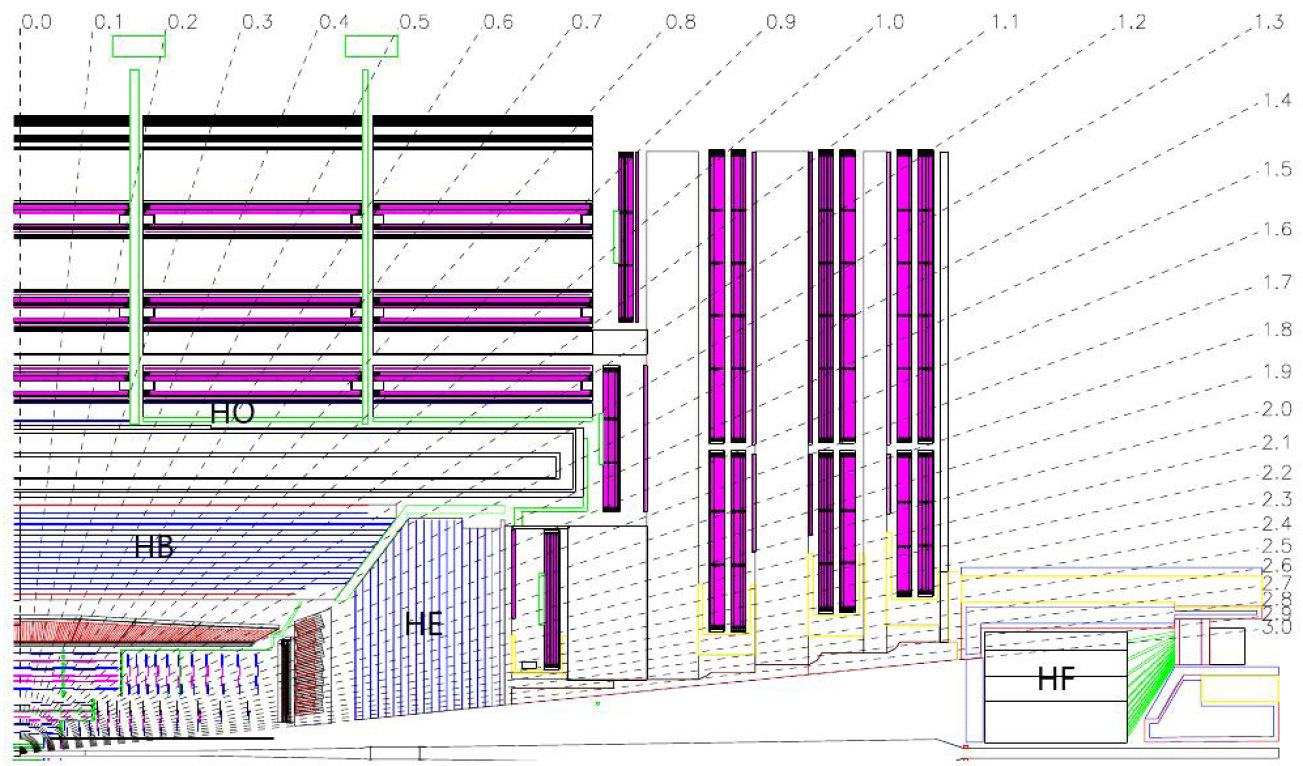
\includegraphics[width=0.9\textwidth]{Figures/detector/cmsHCAL}
  \caption{Longitudinal view of the \ac{CMS} \ac{HCAL}. Locations of the \ac{HB}, \ac{HO}, \ac{HE} and \ac{HF} are shown with values of $\eta$. The purple regions represent the muon detectors which further restrict the volume of the \ac{HO}.
}
  \label{fig:CMShcal}
  \end{center}
\end{figure}

Hadron showers are created in the brass absorber plates, through nuclear interactions in the material, and the plastic scintillator tiles produce blue-violet light when the shower passes through. 
It is read out using wavelength shifting fibres, sending the now green light down transparent fibres to \ac{HPD} which produce an electrical signal proportional to the incident hadron energy.
The first layer of plastic tiles are placed in front of the first absorber plate in order to sample the incoming shower as it develops in the material between the \ac{ECAL} and the \ac{HCAL}.
The final layer of scintillator placed after the final brass plate to catch any late developing showers.
70,000 plastic scintillator tiles are in the \ac{HB} and 20,916 tiles are in the \ac{HE}.

The \ac{HF} uses different technology in order to cope with the much harsher environment in which it is situated.
With an average energy of 760~\GeV deposited in the \ac{HF} per pp collision at LHC design energy, peaking at the highest rapidity point closest to the beam line, radiation hardness and occupancy requirements demand alternative materials.
Steel absorber plates are embedded with scintillating quartz fibres, which act to detect the Cherenkov light emitted by charged particles in the shower. 
It is therefore most sensitive to the electromagnetic component of the shower.


%%%%%%%%%%%%%%%%%%%%%%%%%%%%%%%%%%%%%%%%%%%%%%%%%%%%%%%%%%%%%%%%%%%%%%%%%%%%%%%%%%%%%%%%%%%%%%%

\subsection{The Muon System}
%do i need this
Muons are a powerful tool for recognising signs of interesting physics. 
%Many SUSY models predict excesses of muon decays, for example $B_{s}\rightarrow\mu\mu$, 
%and the Higgs decay $\H \rightarrow \Z\Z$ where both \Z decay to two muons has been called the ``golden plated'' channel.
A relatively easy experimental signature to identify, muons can provide excellent 2- or 4-particle mass resolutions as they do not suffer from radiative losses (as electrons do).
%They are therefore of vital importance to the physics programme at \ac{CMS}, such that they take the middle word of the experiment's name.
Excellent muon reconstruction is therefore a central design feature. 
Embedded in the iron flux-return yoke of the solenoid, the muon systems combine three methods of gaseous detection to identify, carry out high resolution momentum measurements, and trigger events, up to $|\eta|<2.4$.

In the barrel ($|\eta|<0.9$), magnetic flux is concentrated in the iron return yoke so residual field is very small.
There is also a low muon rate and neutron induced background, so \ac{DT} chambers are used.
In the endcaps ($0.9<|\eta|<2.4$), magnetic field and muon rate are much higher, so \ac{CSC} are used instead; 
they have a faster response time, higher granularity and better radiation hardness.
Both the \ac{DT} and \ac{CSC} have excellent position resolution.
An additional system of \ac{RPC} in both the barrel and endcaps provide an independent signal which has both good time resolution (and poorer position resolution) and serves as a trigger.

By combining information from the tracker, and from either the \ac{DT} or \ac{CSC} and \ac{RPC}, ~\ac{CMS} has excellent muon reconstruction. 
Precise momentum resolution is achieved for the whole kinematic range, from 10~\GeV to $>500~\GeV$, shown in  
Figure~\ref{fig:CMSmuonRes}. 

%picture
\begin{figure}[htbp]
  \begin{center}
  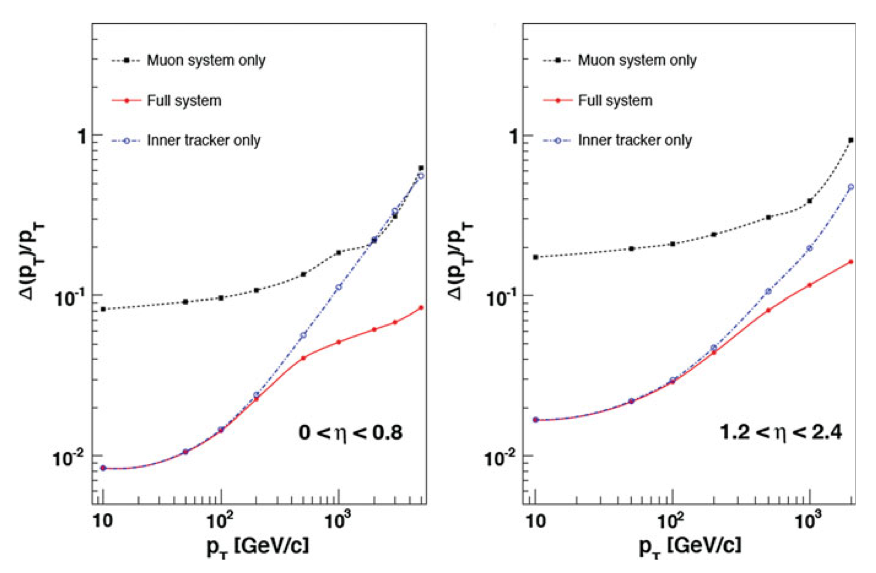
\includegraphics[width=0.9\textwidth]{Figures/detector/CMSmuonRes}
  \caption{Muon transverse momentum resolution, shown as a function of muon \pt in the barrel (left) and the endcaps (right). The resolution of the tracker and muon systems is shown, and the enhancement gained by combining the information.
}
  \label{fig:CMSmuonRes}
  \end{center}
\end{figure}


%%%%%%%%%%%%%%%%%%%%%%%%%%%%%%%%%%%%%%%%%%%%%%%%%%%%%%%%%%%%%%%%%%%%%%%%%%%%%%%%%%%%%%%%%%%%%%%

\subsection{The Trigger}